%%%%%%%%%%%%%%%%%%%%%%%%%%%%%%%%%%%%%%%%%%%%%%%%%%%%%%%%%%%%%%%%%%%%%
%
% Project CV Writeup Template
%
% This is a LaTeX document. LaTeX is a markup language for producing
% documents. Your task is to fill out this
% document, then to compile this into a PDF document.
%
% TO COMPILE:
% > pdflatex thisfile.tex
%
% For references to appear correctly instead of as '??', you must run
% pdflatex twice.
%
%
% If you need help with LaTeX, please come to office hours.
% Or, there is plenty of help online:
% https://en.wikibooks.org/wiki/LaTeX
%
% Good luck!
% Prathmesh and the Proj-CV staff
%
%%%%%%%%%%%%%%%%%%%%%%%%%%%%%%%%%%%%%%%%%%%%%%%%%%%%%%%%%%%%%%%%%%%%%
%
% How to include two graphics on the same line:
%
% \includegraphics[\width=0.49\linewidth]{yourgraphic1.png}
% \includegraphics[\width=0.49\linewidth]{yourgraphic2.png}
%
% How to include equations:
%
% \begin{equation}
% y = mx+c
% \end{equation}
%
%%%%%%%%%%%%%%%%%%%%%%%%%%%%%%%%%%%%%%%%%%%%%%%%%%%%%%%%%%%%%%%%%%%%%%%%%%%%%%%%%%%%%%%%%%%%%%%%

\documentclass[11pt]{article}

\usepackage[english]{babel}
\usepackage[utf8]{inputenc}
\usepackage[colorlinks = true,
            linkcolor = blue,
            urlcolor  = blue]{hyperref}
\usepackage[a4paper,margin=1.5in]{geometry}
\usepackage{stackengine,graphicx}
\usepackage{fancyhdr}
\setlength{\headheight}{15pt}
\usepackage{microtype}
\usepackage{times}
\usepackage{booktabs}
\usepackage{subfigure}
 \usepackage{cite}
% python code format: https://github.com/olivierverdier/python-latex-highlighting
\usepackage{pythonhighlight}

\frenchspacing
\setlength{\parindent}{0cm} % Default is 15pt.
\setlength{\parskip}{0.3cm plus1mm minus1mm}

\pagestyle{fancy}
\fancyhf{}
\lhead{Prathmesh Madhu\\Project 5 Writeup}
\rhead{Project Computer Vision\\
	Summer 2021}
\rfoot{\thepage}

\date{}

\title{\vspace{-1cm}Project 5 Writeup}
\author{Haobo~Song}

\begin{document}
\maketitle
\vspace{-2cm}
\thispagestyle{fancy}

\section*{Project Overview}
In this experiment selective search algorithm \cite{uijlings2013selective} was implemented in practice. And 9 graphs were tested using python code, with relatively good results

\section*{Implement}
The entire selective search is divided into three main steps.
\begin{enumerate}
\item Segment smallest regions \ref{fig:first} by the algorithm of Felzenswalb\cite{felzenszwalb2004efficient}.
\begin{figure}[htbp]
	\centering
				\subfigure[original image]{
		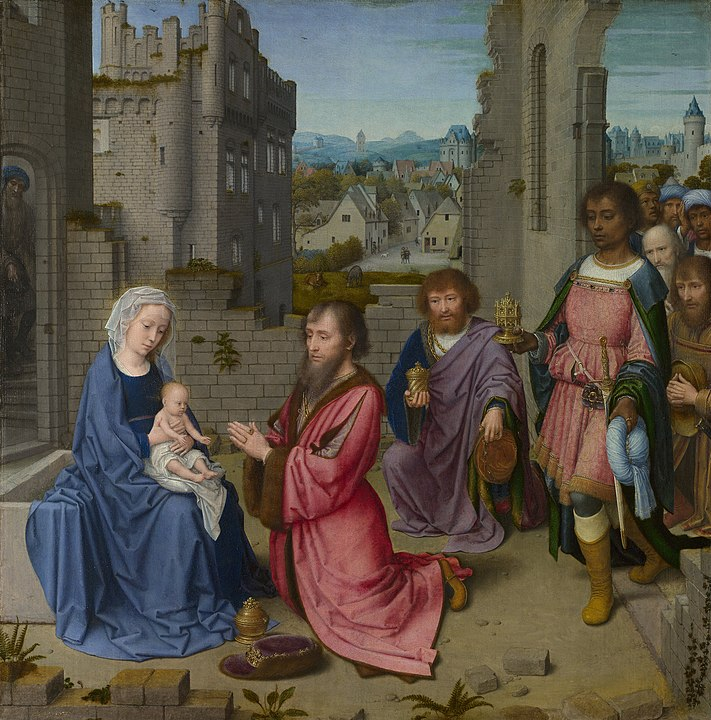
\includegraphics[width=0.3\linewidth]{refe}
	}
		\subfigure[small regions]{
				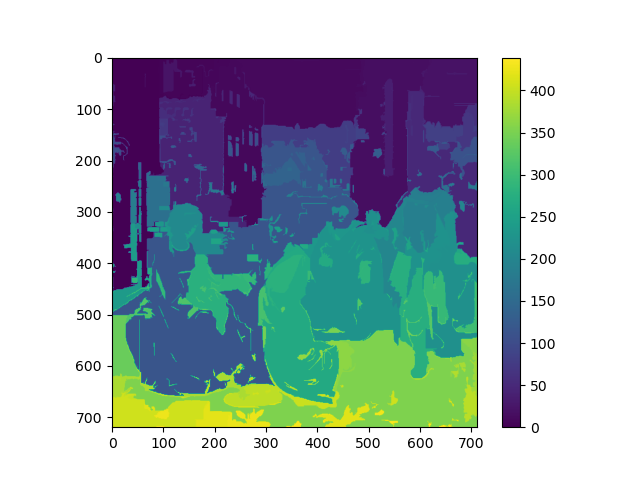
\includegraphics[width=0.5\linewidth]{first}
			}

		\caption{Initialising small regions of the image}
	\label{fig:first}
\end{figure}	
\item Calculate the similarity(color,shape,size,texture) between two regions and merge the two regions with the greatest similarity to obtain a new larger region, which will be added to the region set.
\item Repeat step 2 until there is only one region left, and the resulting set of regions is the output of the algorithm.
\end{enumerate}


\section*{Result}
Following the instructions of the exercise, we implemented the algorithm and obtained the following result \ref{fig:compare_fig}


\begin{figure}[htbp]
	\centering
	\subfigure[image from arthist folder]{
			\centering
			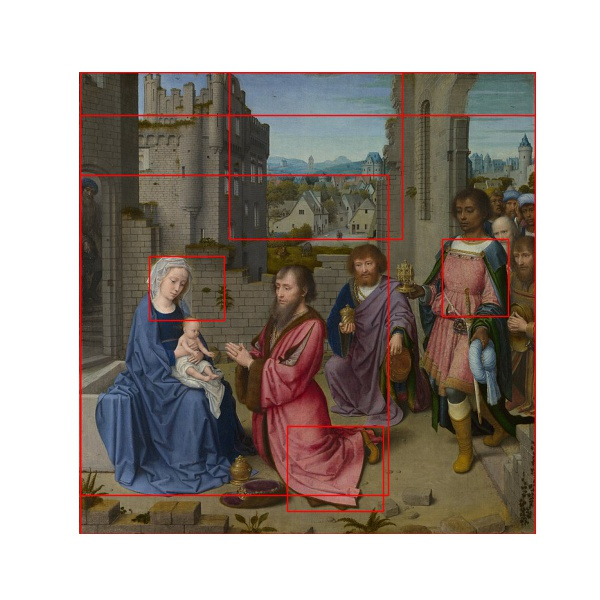
\includegraphics[width=0.33\linewidth]{adoration1}
			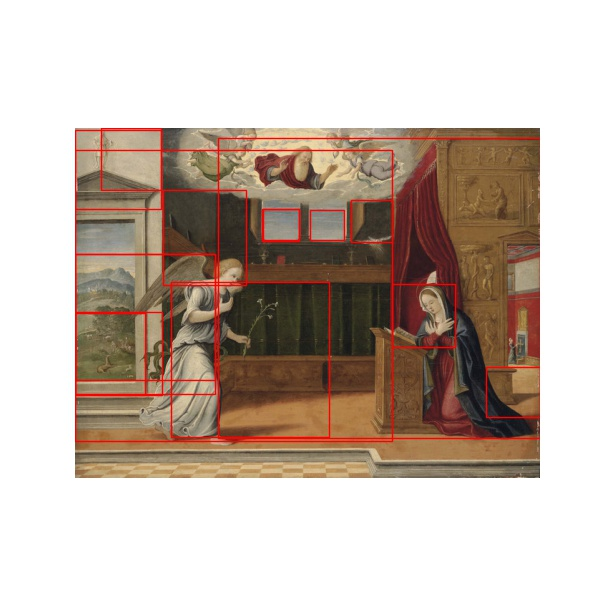
\includegraphics[width=0.33\linewidth]{annunciation1}
			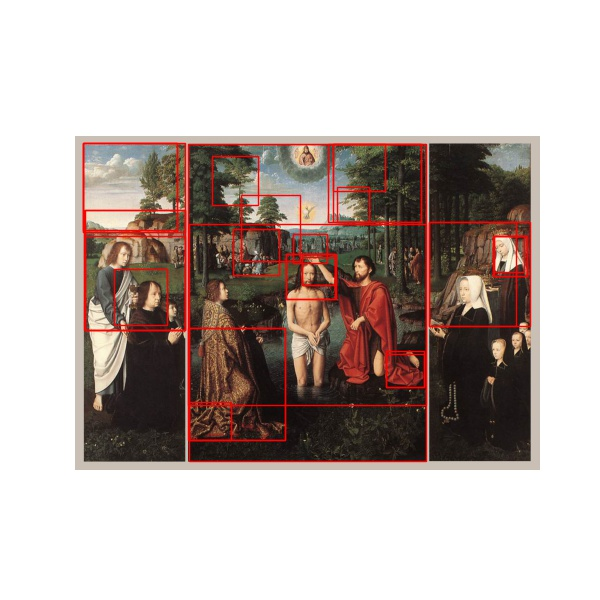
\includegraphics[width=0.33\linewidth]{baptism1}
			%\caption{images from arthist folder}

	}%


	\subfigure[image from chrisarch folder]{

			\centering
			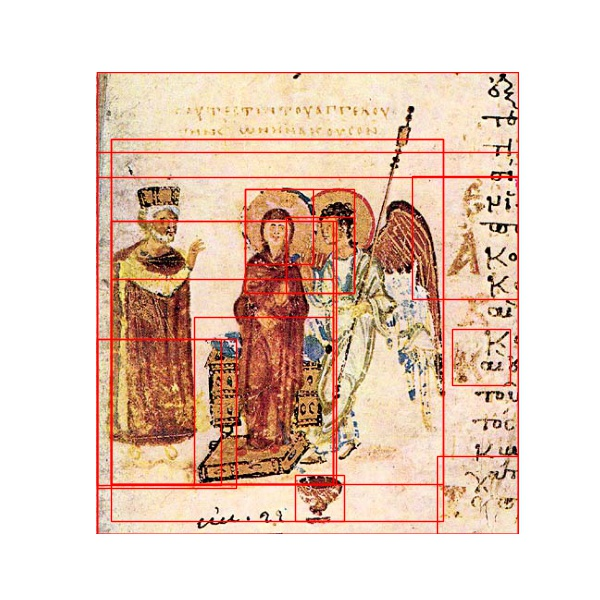
\includegraphics[width=0.33\linewidth]{ca-annun1}
			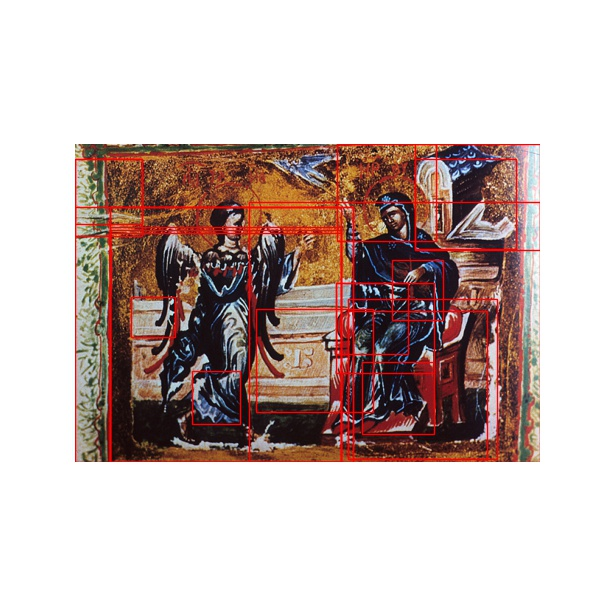
\includegraphics[width=0.33\linewidth]{ca-annun2}
			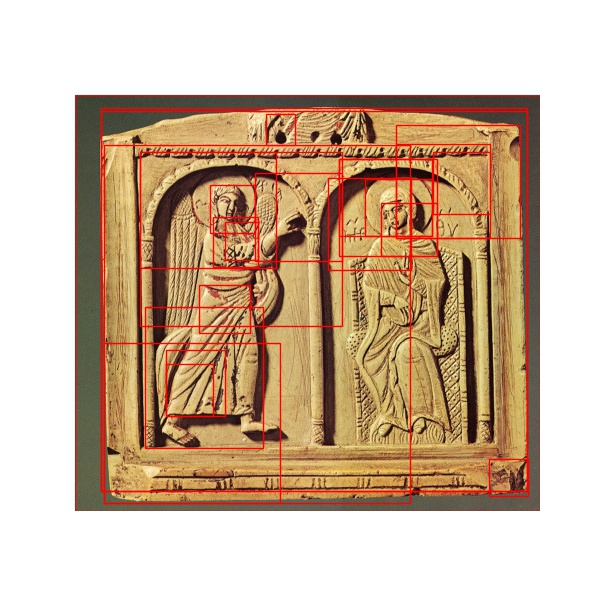
\includegraphics[width=0.33\linewidth]{ca-annun3}

			%\caption{image from chrisarch folder}

	}%
	
	
	\subfigure[image from classarch folder]{
		
		\centering
		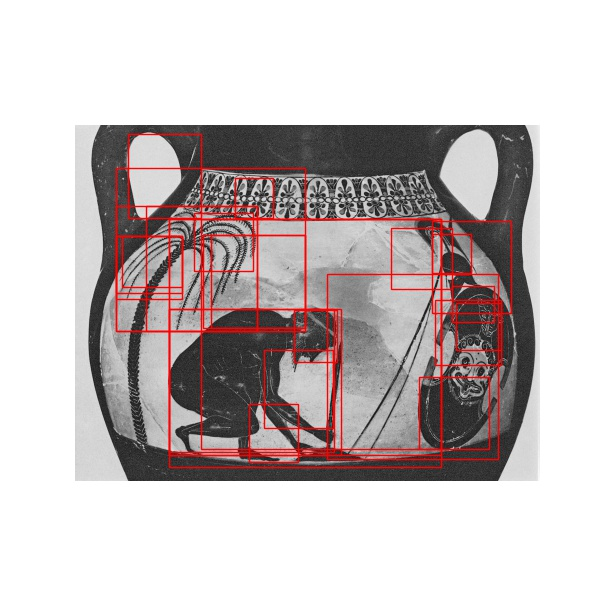
\includegraphics[width=0.33\linewidth]{ajax3}
		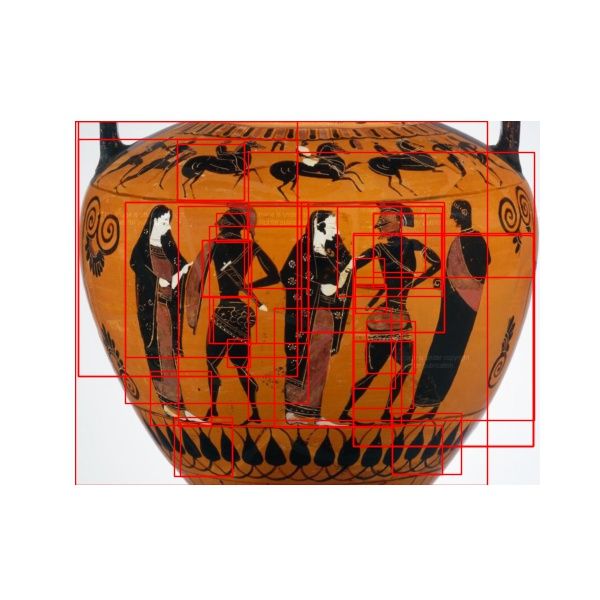
\includegraphics[width=0.33\linewidth]{leading1}
		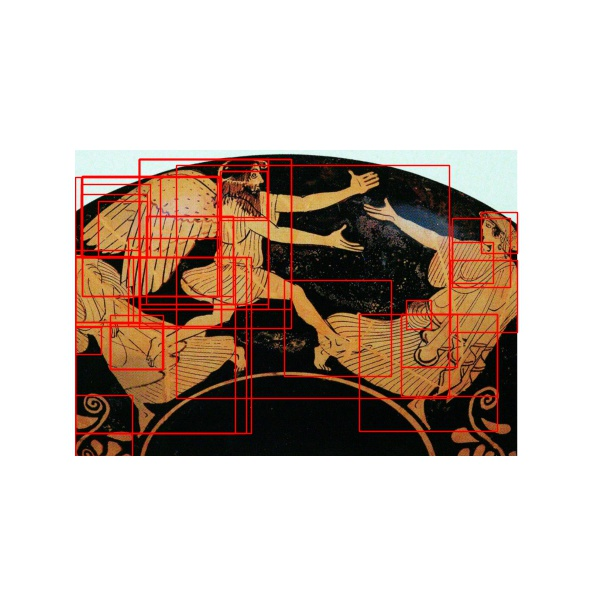
\includegraphics[width=0.33\linewidth]{pursuit2}
		
		%\caption{image from classarch folder}
		
	}%

	\centering
	\caption{Results of all experimental figures}
	\vspace{-0.2cm}
	\label{fig:compare_fig}
\end{figure}

As shown in Figure \ref{fig:compare_fig}, after implementation, all results have reached the expected results.


\section*{Discussion}
For the generation of the final bounding box, we can achieve a preference by giving a weight to the different similarity criteria when measuring the similarity of the regions.

\begin{figure}[htbp]
	\centering
	\subfigure[No change to similarity weights]{
	
	\centering
		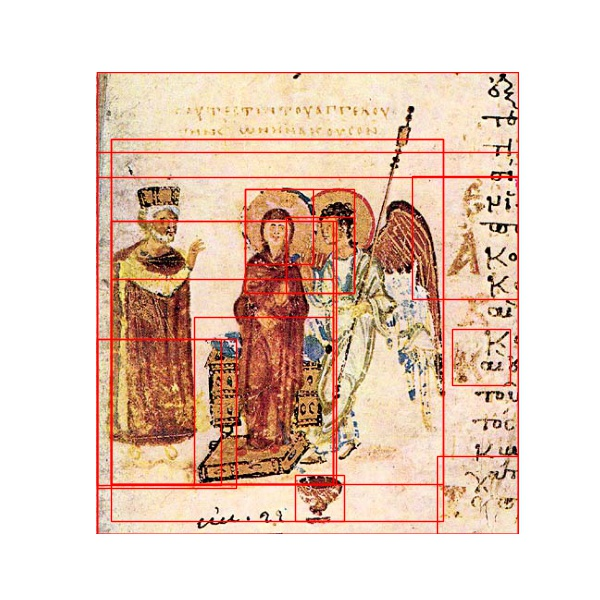
\includegraphics[width=0.4\linewidth]{ca-annun1}
				\label{fig:compare_fig2l}
	
}%
	\subfigure[similarity weights has changed]{
		
		\centering
		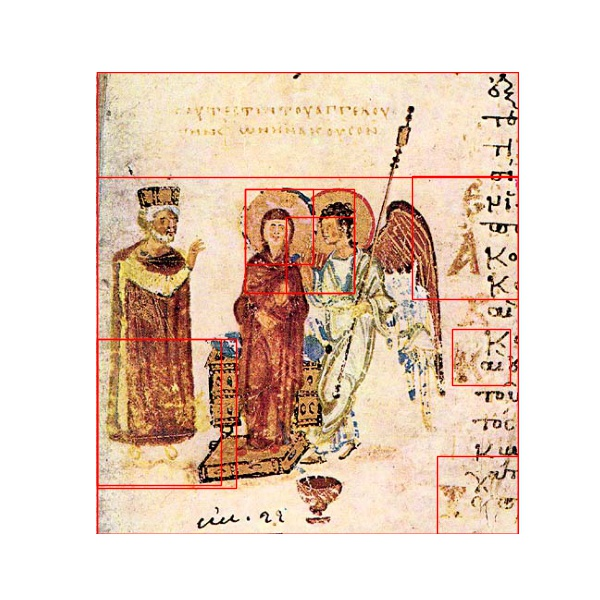
\includegraphics[width=0.4\linewidth]{color_ca-annun1}
			\label{fig:compare_fig2r}
		
	}%

	\centering
	\caption{Different similarity measure weights are used for the same image}
	\vspace{-0.2cm}
	\label{fig:compare_fig2}
\end{figure}

As Figure \ref{fig:compare_fig2} shown above, we have given more weight to the colour similarity and obtained a different bounding box from the original result. As you can see from the right image  \ref{fig:compare_fig2r}, there are fewer bounding boxes than left image \ref{fig:compare_fig2l}, especially in the upper part of the image, where areas of the same colour are divided into a single bounding box. In addition, As shown in the figure below \ref{fig:compare_fig3} the sensitivity to small object detection can be improved by modifying the size threshold of the smallest bounding box, but usually he also produces more redundant bounding boxes.
\begin{figure}[htbp]
	\centering
	\subfigure[No change to size threshold]{
		
		\centering
		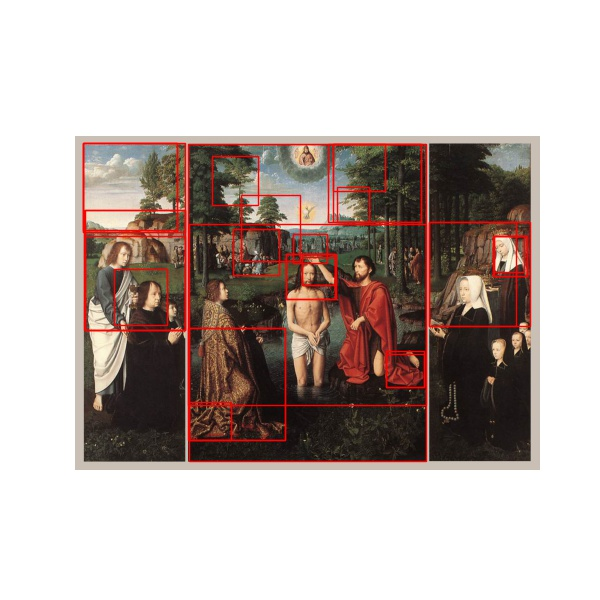
\includegraphics[width=0.4\linewidth]{baptism1}
		\label{fig:compare_fig3l}
		
	}%
	\subfigure[size threshold has changed]{
		
		\centering
		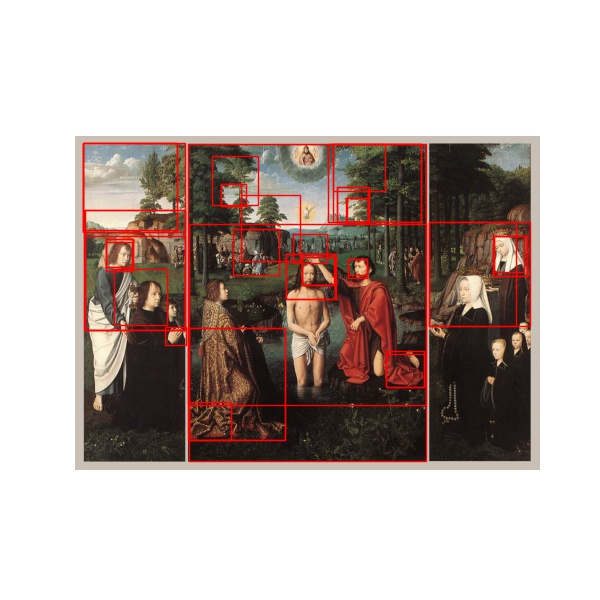
\includegraphics[width=0.4\linewidth]{size_baptism1}
		\label{fig:compare_fig3r}
		
	}%
	
	\centering
	\caption{Different size threshold are used for the same image}
	\vspace{-0.2cm}
	\label{fig:compare_fig3}
\end{figure}

We can conclude that with the selective search algorithm, we can quickly do a pre-processed segmentation of the image and get a lot of regions of interest, but the detail is not ideal . Segmentation in detail requires parameter adjustment or other algorithms


\bibliographystyle{IEEEtran}

\bibliography{wr}
\end{document}
